\documentclass{beamer}
\usepackage[english]{babel}
\usepackage[utf8]{inputenc}
\usepackage{multicol}
\usepackage{graphicx}
\usepackage{subfig}
\usepackage{hyperref}
\hypersetup{
    colorlinks=true,
    linkcolor=blue,
    filecolor=magenta,      
    urlcolor=blue,
}
%\usepackage[shortlabels]{enumitem}
\usepackage{amsmath,amsthm, amssymb, latexsym}

\usetheme{Frankfurt}
\usefonttheme[onlymath]{serif}
\setbeamertemplate{caption}[numbered]
\setbeamertemplate{enumerate items}[default]
\setbeamertemplate{bibliography item}{\insertbiblabel}
\usepackage[orientation=landscape, size=a0]{beamerposter}

\usepackage[absolute, overlay]{textpos}
\setlength{\TPHorizModule}{\paperwidth}
\setlength{\TPVertModule}{\paperheight}

\title{\huge Boundary Effects in Stochastic Cyclic Competition Models on a Two-Dimensional Lattice}
\author{\Large M. Lazarus Arnau, Shannon Serrao, Uwe C. T{\"a}uber}
\institute{\normalsize Department of Physics (MC 0435) and Center for Soft Matter and Biological Physics\\ Virginia Tech, Blacksburg, Virginia 24061}
\date{July 26, 2018}

\begin{document}
\begin{frame}{}

%Left Col
\begin{textblock}{0.32}(0.01,0.015)
    \begin{block}{Introduction}
        \begin{figure}[h]
            \centering
            \subfloat[]{{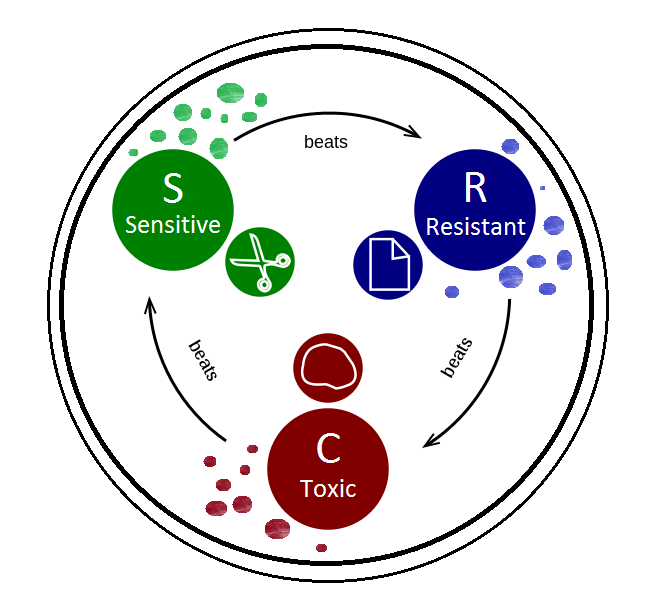
\includegraphics[width=0.4\linewidth]{images/ecolirps.png} }}
            \subfloat[]{{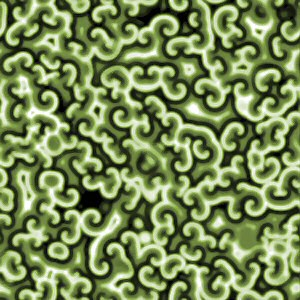
\includegraphics[width=0.4\linewidth]{images/Belousov-Zhabotinsky.jpg} }}
            \caption{(a) Cyclic dominance in \textit{E. coli} (b) Spiral pattern formation in the Belousov-Zhabotinsky reaction.}
            \label{fig:images}
        \end{figure}
        A number of systems in the fields of ecology, epidemiology, and chemistry
        follow a paradigm of cyclic dominance or have been shown to exhibit noise-induced 
        pattern formation (e.g. certain subspecies of Lizards in
        California \cite{sinervo96}, experiments on cyclically competing \textit{E. coli} bacteria \cite{kerr02}, and
        the Belousov-Zhabotinsky reaction \cite{epstein96}). The formation of noise-induced and -stabilized
        spiral patterns in this class of system is captured by the spatially-extended 
        May-Leonard (ML) model. The formation of these spirals is in stark contrast
        to the species clustering seen in the Rock-Paper-Scissors (RPS) model.        
    \end{block}
    \hfill
    \begin{block}{The RPS Model}
        The RPS Model is defined by the following binary reactions:
        \begin{itemize}
            \item Replacement reaction:
            \begin{gather*}
                AB \rightarrow AA\\
                BC \rightarrow BB\\
                CA \rightarrow CC\\            
                \text{with rate } \zeta
            \end{gather*}

            \item Pair swap / diffusion reaction:
            \begin{gather*}
                XY \rightarrow YX \\
                \text{where }X, Y \in \{A, B, C, \varnothing\} \text{ with rate } \epsilon_r
            \end{gather*}
        \end{itemize}
    \end{block}
    \hfill
    \begin{block}{The May-Leonard Model}
        The ML Model is defined by the following binary reactions:
        \begin{itemize}
            \item Predation reaction:
            \begin{gather*}
                AB \rightarrow A \varnothing \\
                BC \rightarrow B \varnothing \\
                CA \rightarrow C \varnothing \\            
                \text{with rate } \sigma
            \end{gather*}
            \item Reproduction reaction:
            \begin{gather*}
                A \varnothing \rightarrow AA\\
                B \varnothing \rightarrow BB\\
                C \varnothing \rightarrow CC\\            
                \text{with rate } \mu
            \end{gather*}
            \item Pair swap / diffusion reaction:
            \begin{gather*}
                XY \rightarrow YX \\
                X, Y \in \{A, B, C, \varnothing\} \text{ with rate } \epsilon_m
            \end{gather*}
        \end{itemize}

    \end{block}
    \hfill
    \begin{block}{Simulation}
        We define $x$ to be the vertical (short) axis and $y$ to be the horizontal
        (long) axis. A lattice of size $L_x \times L_y$ is then initialized with each cell 
        being assigned a random species with probability $p (A) = p (B) = p (C) = {\rho_0}/{3}$ (where $\rho_0$ is the 
        initial net particle density). We limit each lattice point to contain at most
        one particle.
        The lattice is given a toroidal topology (i.e. $x=0 \text{ is equivalent 
        to } x = L_x$ and likewise for $y = L_y$). The simulation then proceeds according 
        to the following algorithm:

        \begin{enumerate}
            \item A random coordinate $(x, y)$ is selected from a uniform distribution
                and time is advanced by $\delta t = N^{-1} $ (where $N = L_x \times L_y$).
            \item If that lattice point is not empty, then a nearest neighbor is chosen
                at random. If the cell is empty, the simulation returns to step 1.
            \item One of the possible reactions (according to whether the lattice point
                is governed by the ML or RPS model) is selected at random, and excecuted
                if possible. The simulation returns to step 1.
        \end{enumerate}

        In cases where there are both RPS and ML lattice points, all lattice points
        in the range $0 \leq y < d_i$ are governed by the RPS model and all 
        remaining lattice points are governed by the ML model.
    \end{block}
\end{textblock}

%Middle Collumn
\begin{textblock}{0.32}(0.34, 0.0125)
    \begin{block}{}
        \maketitle
        \centering
        We study noise-induced and -stabilized spatial patterns in two distinct stochastic 
        population model variants for cyclic competition of three species, namely the 
        Rock-Paper-Scissors (RPS) and the May-Leonard (ML) models. In two dimensions, 
        it is well established that the ML model can display (quasi-)stable spiral 
        structures, in contrast to simple species clustering in the RPS system. Our 
        ultimate goal is to impose control over such competing structures in systems 
        where both RPS and ML reactions are implemented. To this end, we have employed 
        Monte Carlo computer simulations to investigate how changing the microscopic 
        rules in a subsection of a two-dimensional lattice influences the macroscopic 
        behavior in the rest of the lattice. Specifically, we implement the ML reaction scheme 
        on a torus, except on a ring-shaped patch, which is set to follow the cyclic 
        Lotka-Volterra predation rules of the RPS model. There, we observe a marked disruption of 
        the usual spiral patterns in the form of plane waves emanating from the RPS region, 
        up to a characteristic distance that is set by the diffusion rate in the RPS 
        patch. Furthermore, the overall population density drops considerably in the 
        vicinity of the interface between both regions. 
    \end{block}
    \hfill
    \begin{block}{Normal Pattern Formation}
        \begin{figure}[h]
            \centering
            \subfloat[$\epsilon_m=0.1$]{{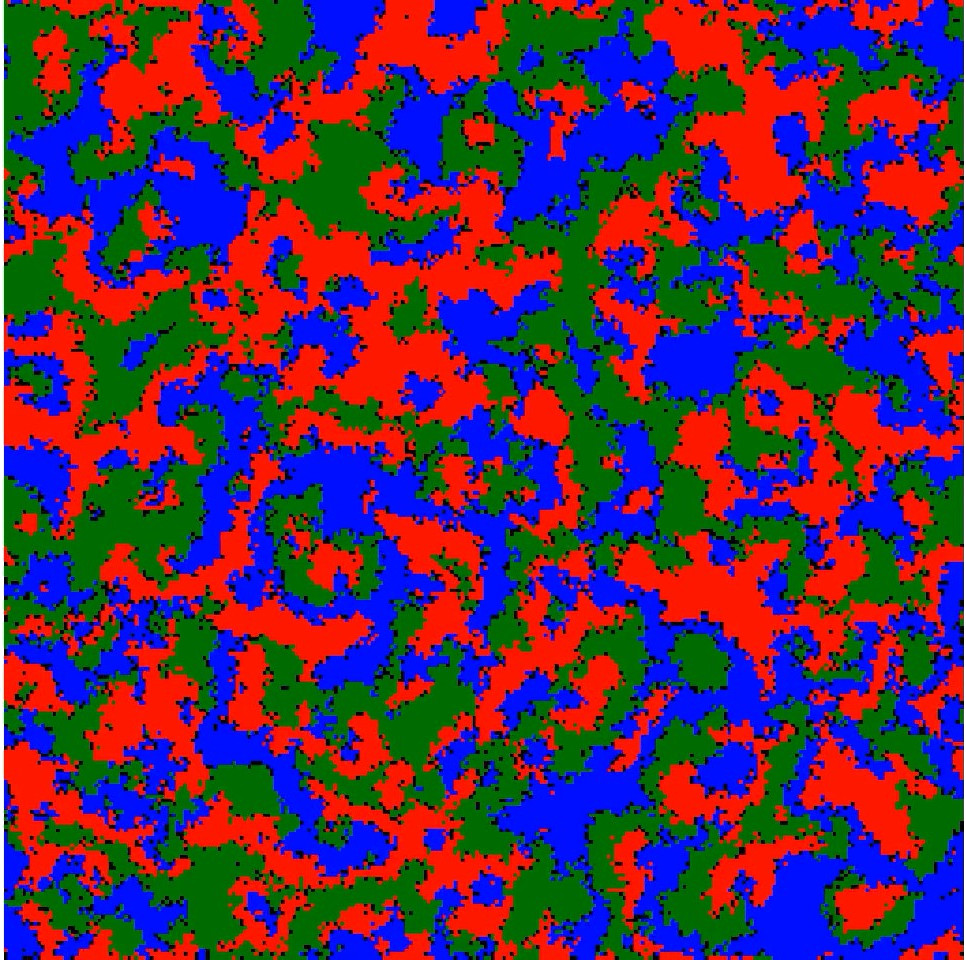
\includegraphics[width=0.24\linewidth]{images/ml_0_1.jpg} }}
            \subfloat[$\epsilon_m=1.25$]{{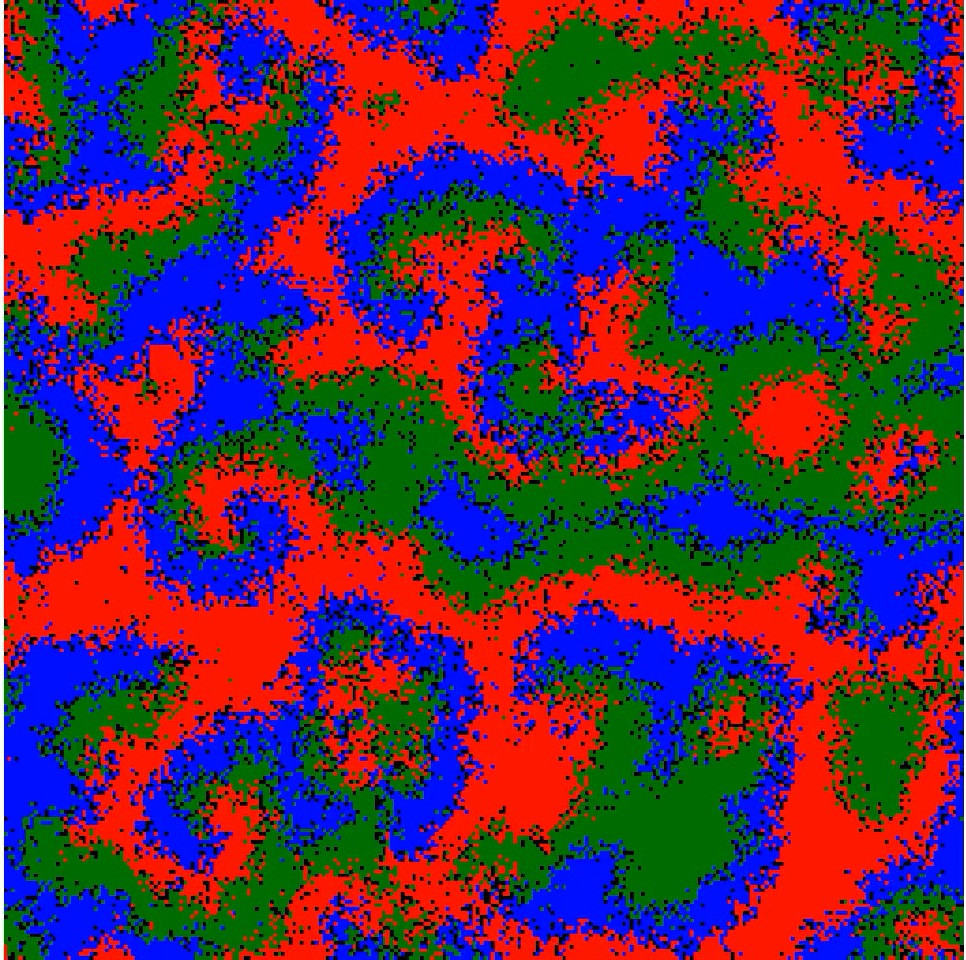
\includegraphics[width=0.24\linewidth]{images/ml_1_25.jpg} }}
            \subfloat[$\epsilon_m=5.0$]{{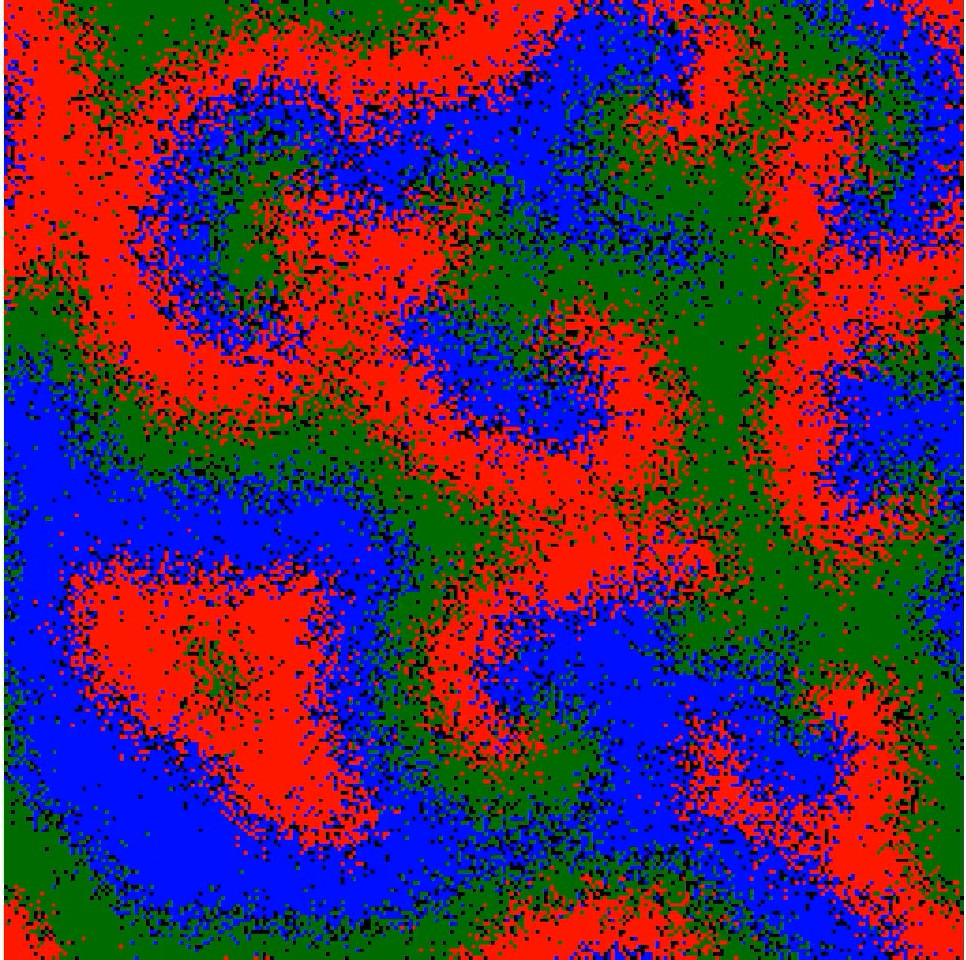
\includegraphics[width=0.24\linewidth]{images/ml_5_0.jpg} }}
            \subfloat[$\epsilon_m=10.0$]{{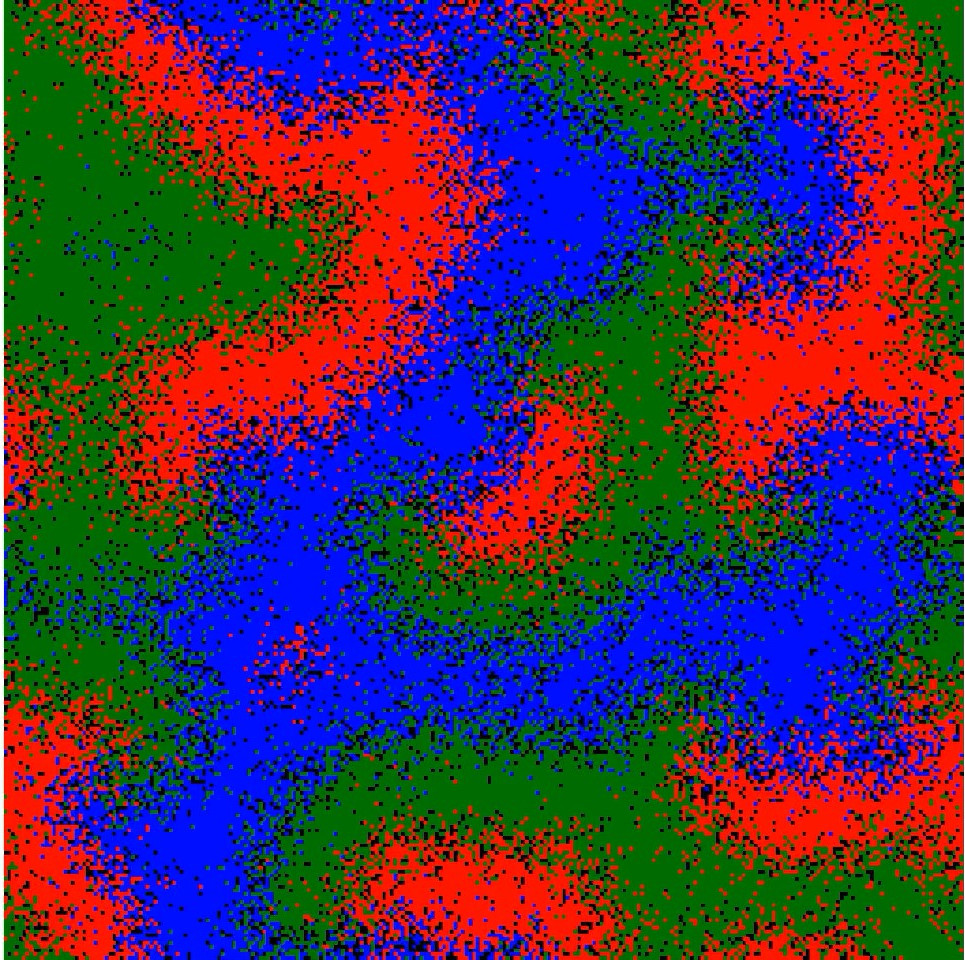
\includegraphics[width=0.24\linewidth]{images/ml_10_0.jpg} }}
            \\
            \subfloat[$\epsilon_r=0.1$]{{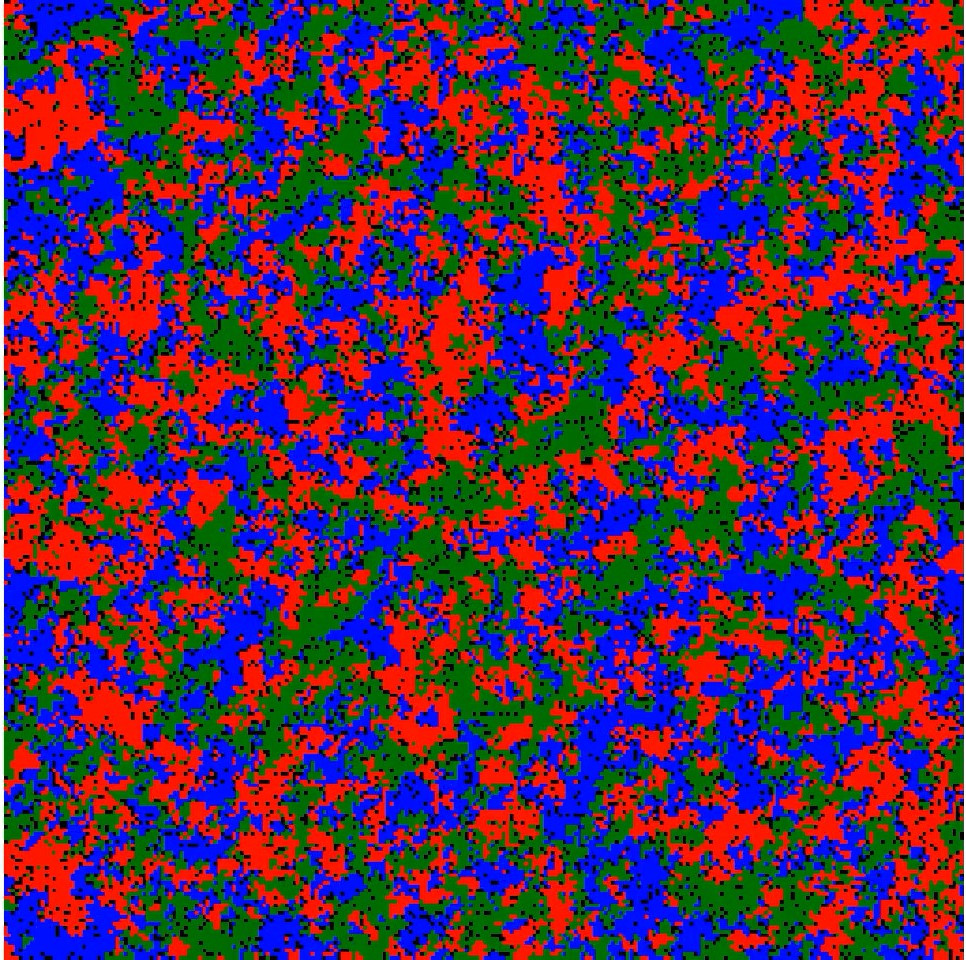
\includegraphics[width=0.24\linewidth]{images/rps_0_1.jpg} }}
            \subfloat[$\epsilon_r=1.25$]{{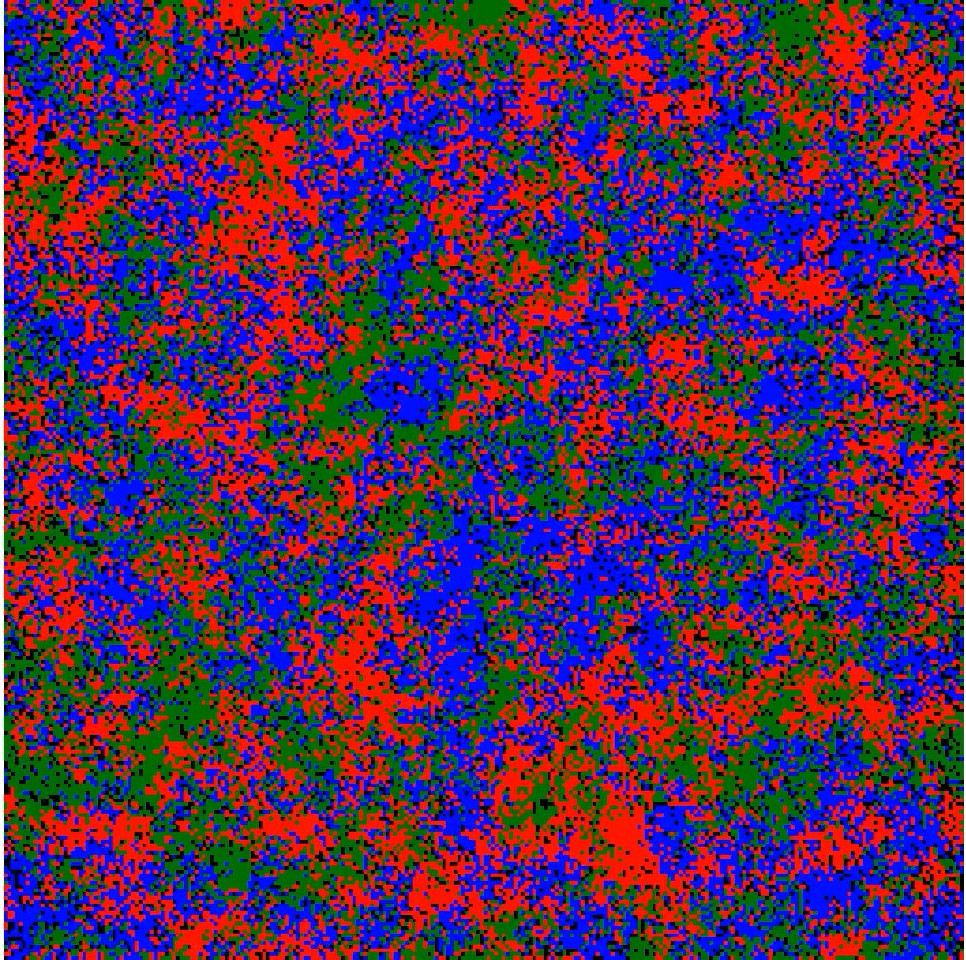
\includegraphics[width=0.24\linewidth]{images/rps_1_25.jpg} }}
            \subfloat[$\epsilon_r=5.0$]{{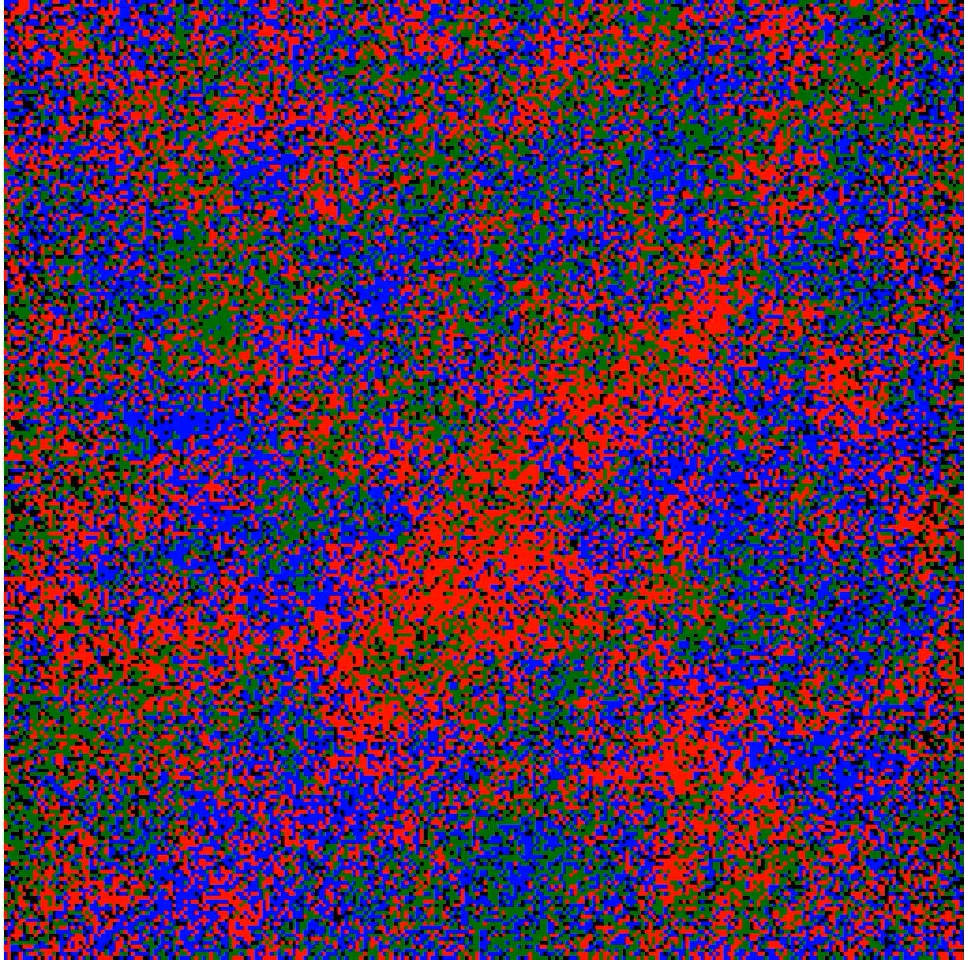
\includegraphics[width=0.24\linewidth]{images/rps_5_0.jpg} }}
            \subfloat[$\epsilon_r=10.0$]{{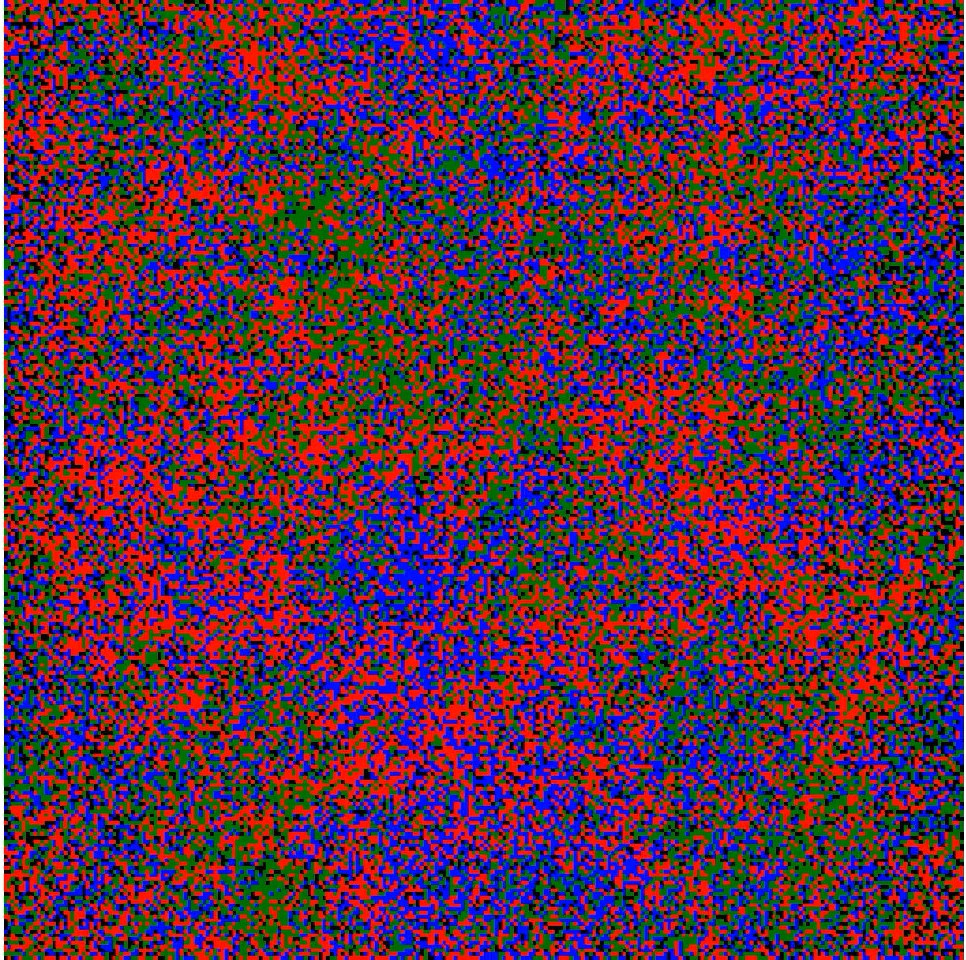
\includegraphics[width=0.24\linewidth]{images/rps_10_0.jpg} }}
            \caption{\centering Steady state snapshots. All lattices have $L_x = L_y = 256$: \\ (a)-(d) Typical ML pattern formation. $\sigma = \sigma = \mu = 1.0$  (e)-(h) Typical RPS pattern formation. $\zeta = 1.0$.}
            \label{fig:patterns}
        \end{figure}
        Our simulations produce (quasi-)stable patterns similar to those seen by Qian He \textit{et al.} \cite{he2011} and Peltom{\"a}ki and Alava \cite{peltomaki08}.

    \end{block}
    \hfill
    \begin{block}{Plane Wave Formation}
        \begin{figure}[h]
            \centering
            \subfloat[$\epsilon_m=0.1$]{{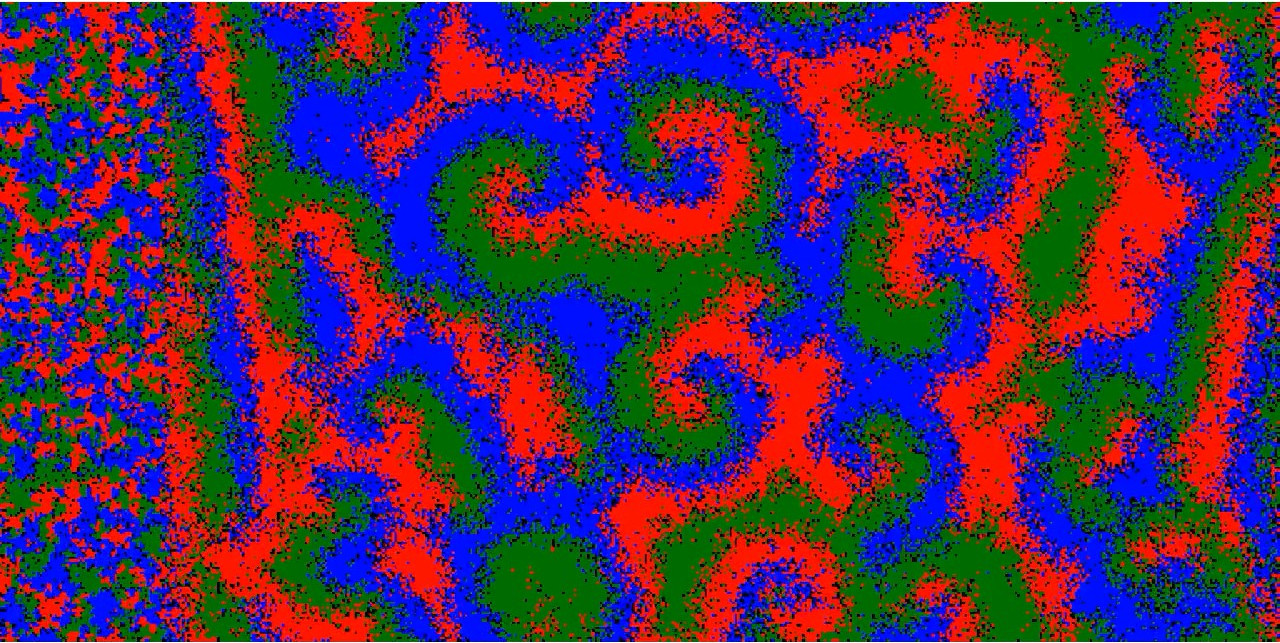
\includegraphics[width=0.48\linewidth]{images/mlrps_0_1.jpg} }}
            \subfloat[$\epsilon_m=2.5$]{{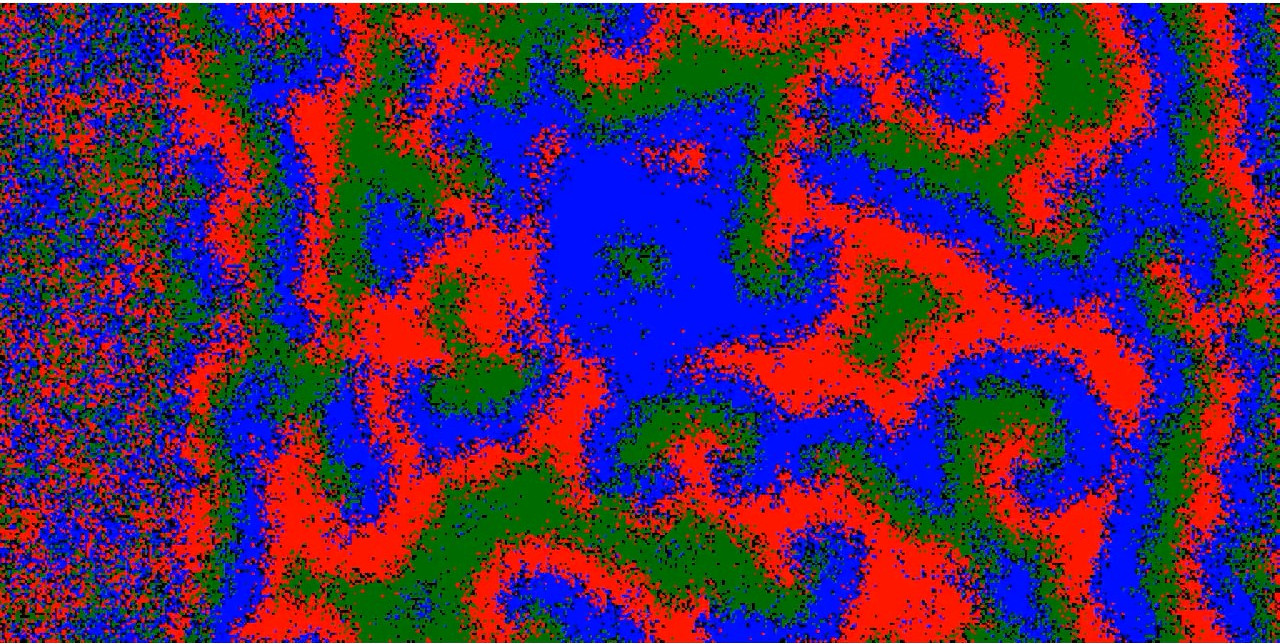
\includegraphics[width=0.48\linewidth]{images/mlrps_2_5.jpg} }}
            \\
            \subfloat[$\epsilon_m=5.0$]{{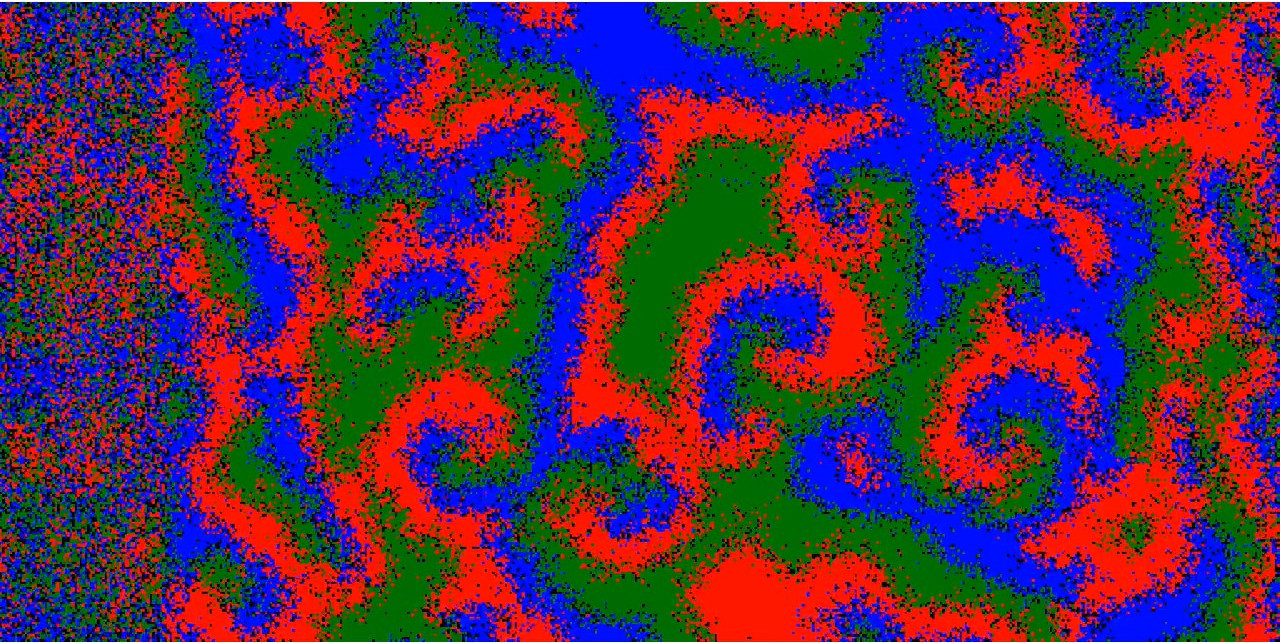
\includegraphics[width=0.48\linewidth]{images/mlrps_5_0.jpg} }}
            \subfloat[$\epsilon_m=10.0$]{{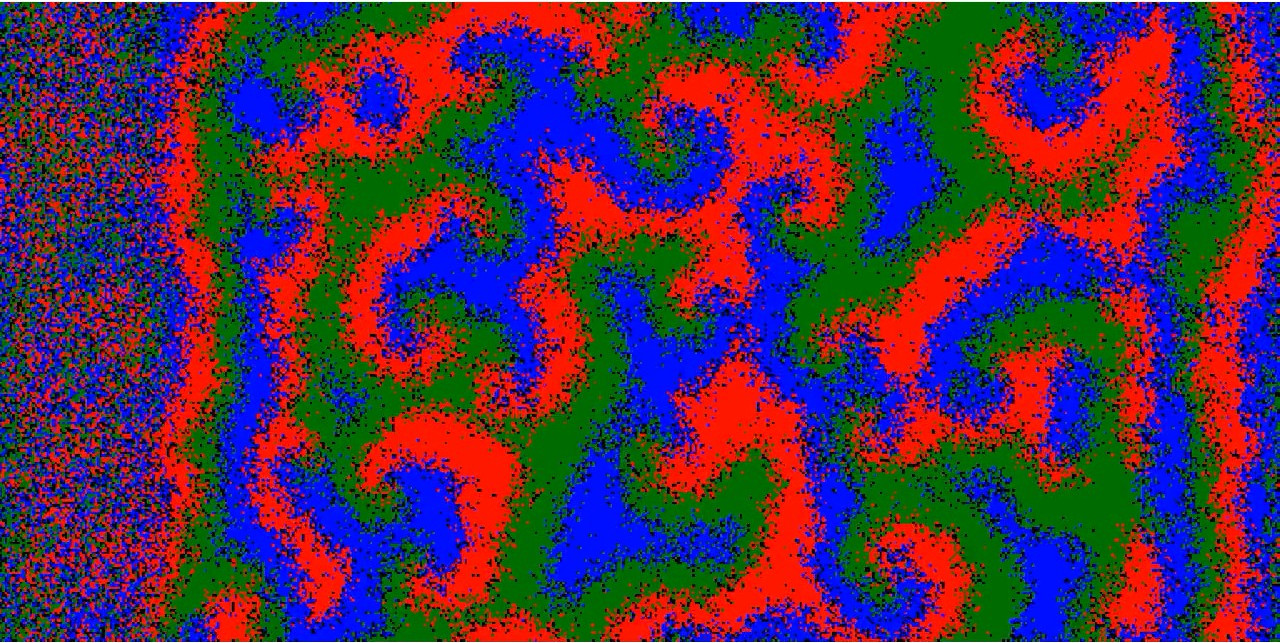
\includegraphics[width=0.48\linewidth]{images/mlrps_10_0.jpg} }}
            \caption{\centering Steady state snapshots of plane wave formation in $256 \times 512$ lattices. In all cases $\epsilon_m = 2.5, \ \sigma = \mu = 1.0, \ \zeta = 1.0$. The interface is placed at $y = 64$.}
            \label{fig:plane_waves}
        \end{figure}
    \end{block}
    \hfill
    \begin{center}
        
\includegraphics[width=0.25\linewidth]{images/vt_logo.jpg}
    \end{center}
    \hfill
\end{textblock}

\begin{textblock}{0.32}(0.67,0.015)
    %\begin{block}{Characteristic Dynamics of the ML Model}
    %The following values were derived analytically by \textit{Reichenbach, et. al.} \cite{reichenbach08} 
    %\begin{align*}
    %\text{Diffusion Constant:} \quad & D = \epsilon_m d^{-1} N^{-2 / d} \\
    %\quad & \text{where } d \text{ is the number of spatial dimensions}\\
    %\quad & \text{and } N \text{ is the size of the lattice.}\\
    %\text{Constants:} \quad & c_1 = \frac{1}{2}\frac{\mu\sigma}{3\mu + \sigma}, \quad  c_3 = \frac{\sqrt{3}\left(18\mu + 11\sigma\right)}{48\mu + 11\sigma}\\
    %\text{Spreading Velocity:} \quad & v^* = 2 \sqrt{c_1 D}\\
    %\text{Wavelength:} \quad & \lambda = \frac{2\pi c_3 \sqrt{D}}{\sqrt{c_1}\left(1 - \sqrt{1 + c_3^2}\right)}\\
%\end{align*}
    %
    %We use these values to contextualize our measurements in the next section.
    %For the cases shown below we use $d=2$ and $N = W \times H = 2^{17},$ 
    %$\sigma = \mu = \zeta = 1.0 , \text{ and } \epsilon_m = 2.5$
        %This yields theoretical values of $D \approx 9.5 \times 10^{-6}$, $ v^* 
        %\approx 0.00218$, and $ \lambda \approx 0.18$
    %\end{block}
    \begin{block}{Plane Wave Behavior:}
        \begin{center}
            \begin{tabular}{c|c|c}
                $\epsilon_m$    & $d_p$ & $v $       \\%& $2 \tau v$ \\
                \hline 
                0.01            & 0.119 & 0.000198  \\%& 0.00178\\
                2.5             & 0.168 & 0.000206  \\%& 0.00185\\
                5.0             & 0.168 & 0.000192  \\%& 0.00173\\
                10.0            & 0.129 & 0.000194  \\%& 0.00175\\
            \end{tabular}
        \end{center}
        Using plots of density measured parallel to the interface, we visually
        estimate the permeation distance ($d_p$) and front velocity ($v$)
        of the plane waves. Reichenbach \textit{et al.} \cite{reichenbach08} showed
        that the wave front velocity in the May-Leonard model is determined by the 
        reaction rates. Unsurprisingly, we see that $v$ stays (approximately) constant across our simulations.
        We also find that $d_p$ seems to be, at least in part, dependant on $\epsilon_r$,
        reaching a maximum when $\epsilon_r$ is close to $\epsilon_m$. 
        %We also rescale velocity by $2 \tau$ (where $\tau = \epsilon_m + \sigma + \mu$)
        %in order to account for differences in how Reichenbach, \textit{et. al.} \cite{reichenbach08} handle time scaling.
        %Note that their numerical results for spreading velocity also deviate from
        %their analytical result by $ \approx 10 \%$. We thus see that, unsurprisingly,
        %plane waves travel at approximately the characteristic spreading velocity of 
        %the system. 
    \end{block}
    \begin{block}{Interface Density Effects}
        \begin{figure}[h]
            \centering
            \subfloat[$\epsilon_m=0.1$]{{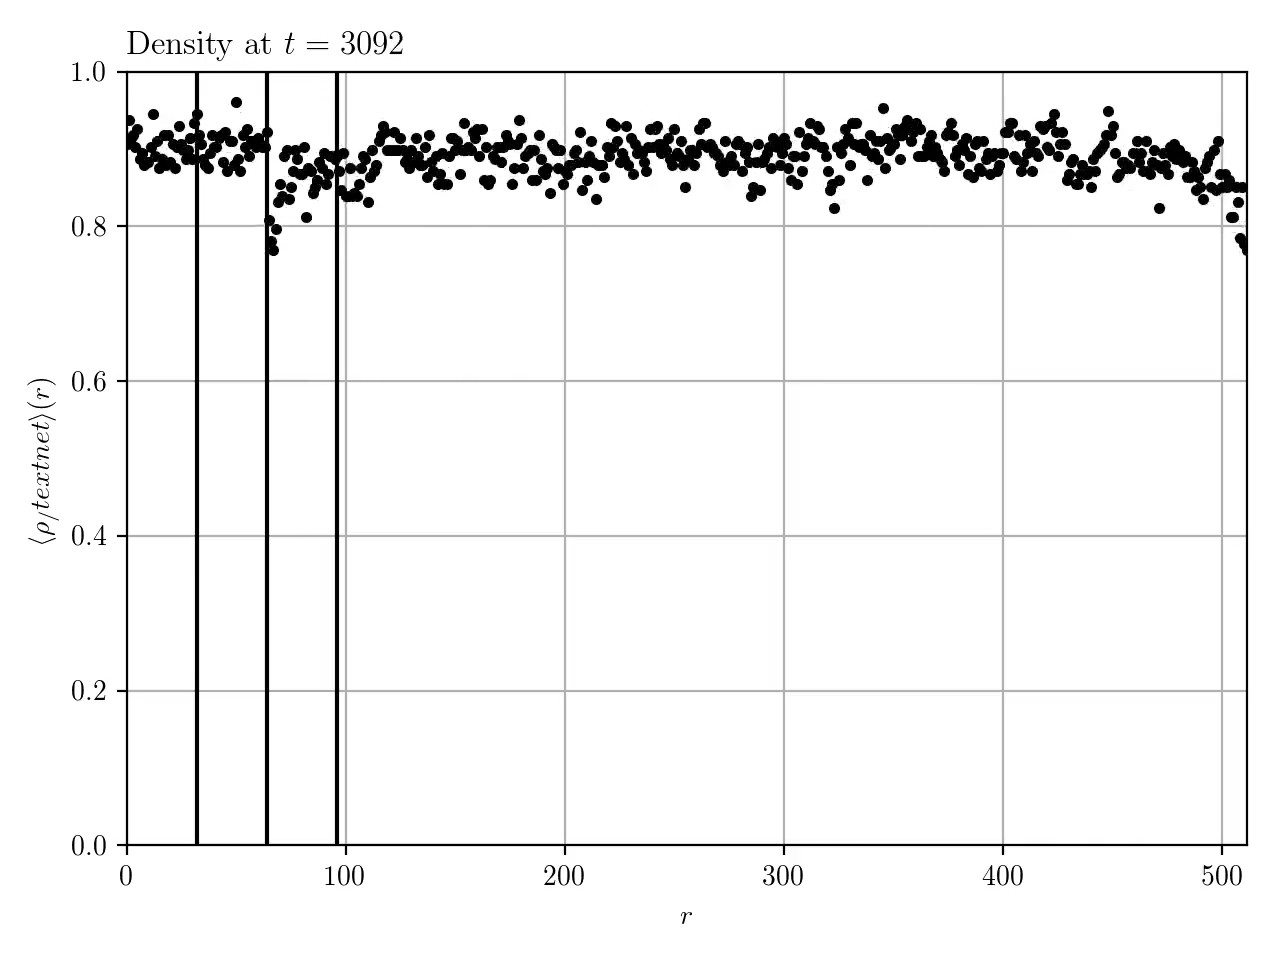
\includegraphics[width=0.4\linewidth]{images/net_density_0_1.jpg} }}
            \subfloat[$\epsilon_m=2.5$]{{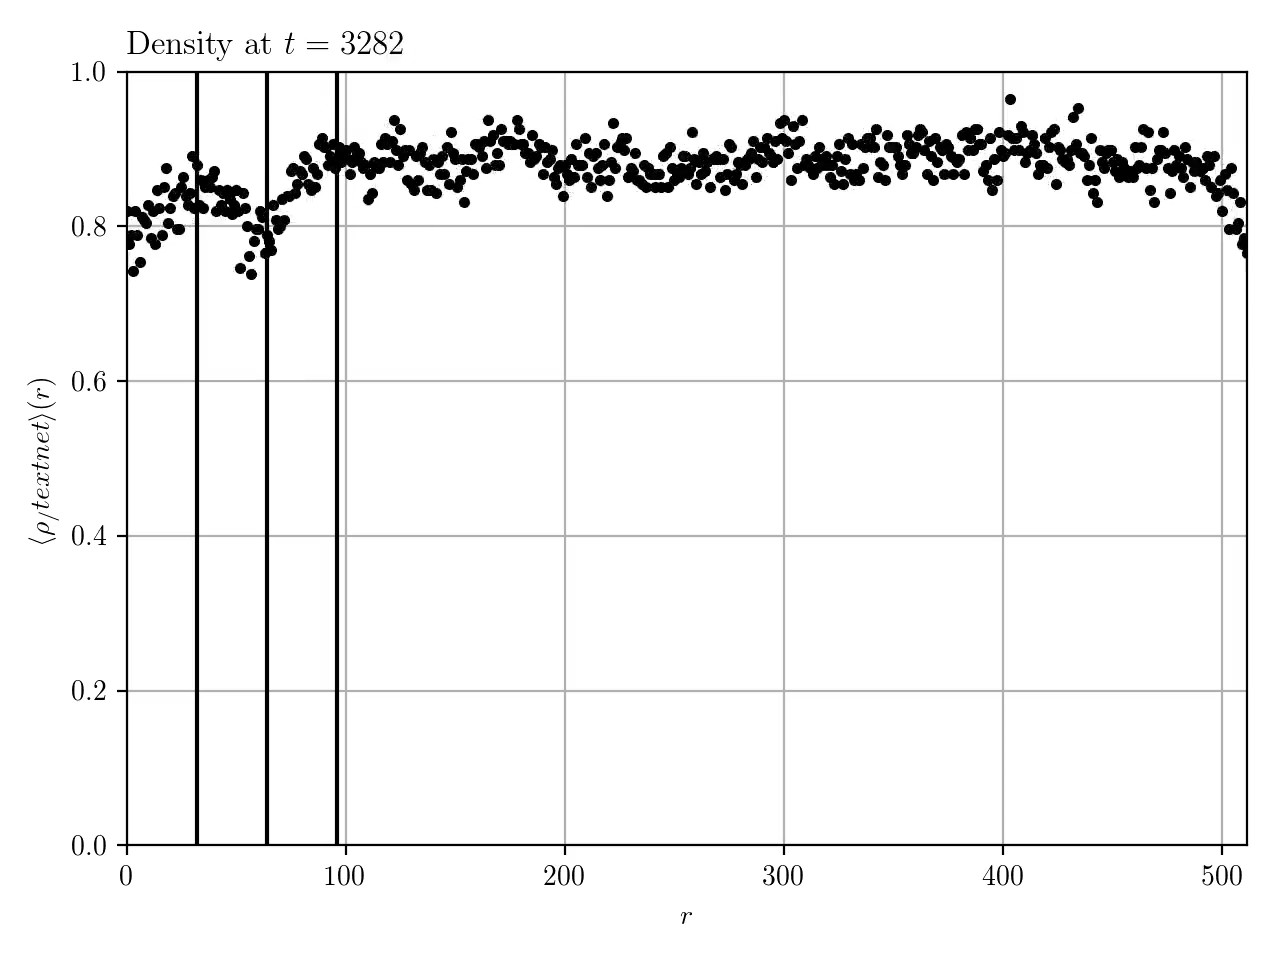
\includegraphics[width=0.4\linewidth]{images/net_density_2_5.jpg} }}
            \\
            \subfloat[$\epsilon_m=5.0$]{{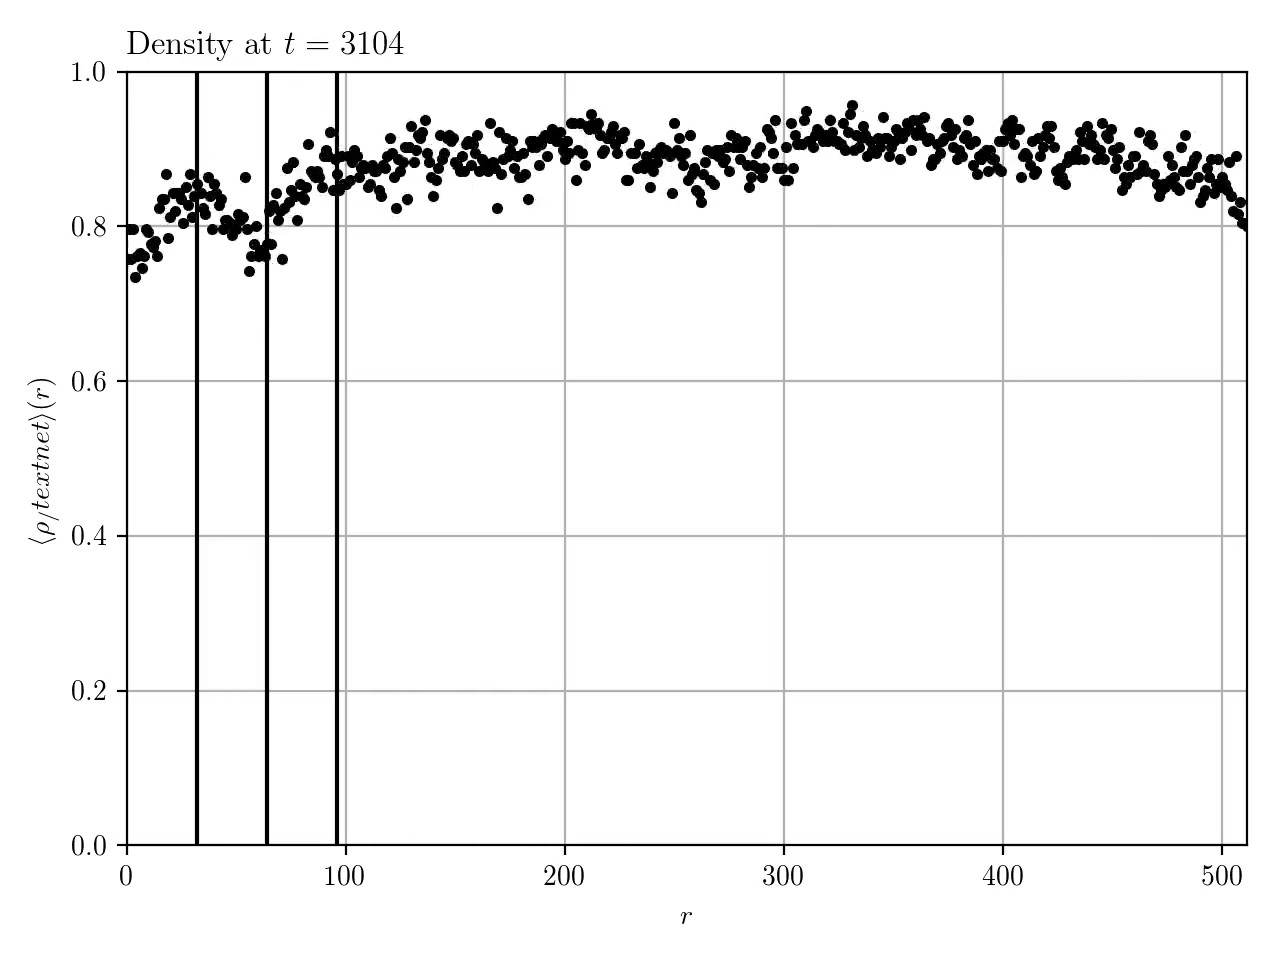
\includegraphics[width=0.4\linewidth]{images/net_density_5_0.jpg} }}
            \subfloat[$\epsilon_m=10.0$]{{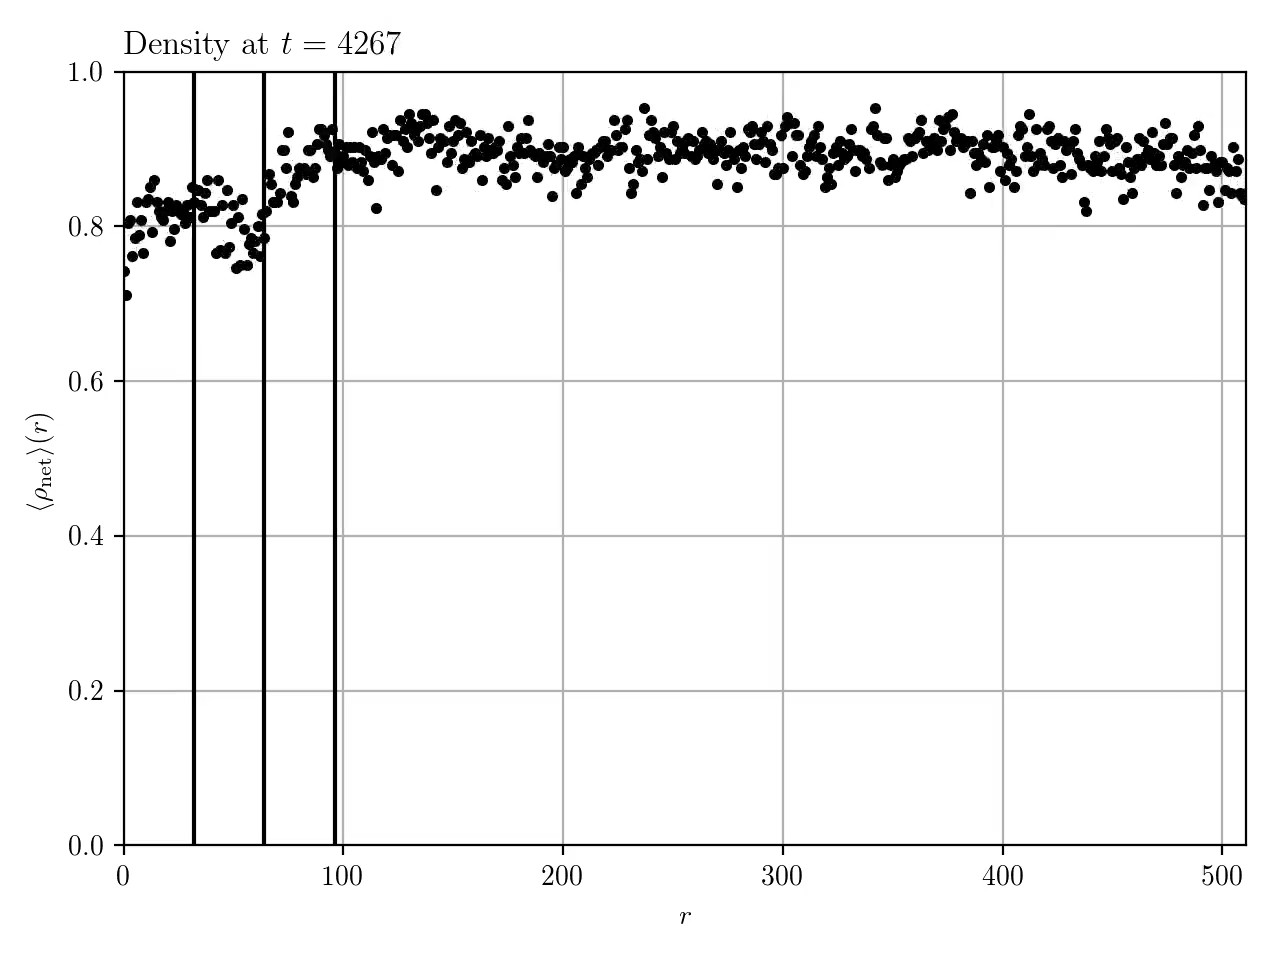
\includegraphics[width=0.4\linewidth]{images/net_density_10_0.jpg} }}
            \caption{\centering Plane wave formation in $256 \times 512$ lattices. In all cases $\epsilon_m = 2.5, \ \sigma = \mu = 1.0, \ \zeta = 1.0$. The interface is placed at $y = 64$.}
            \label{fig:void}
        \end{figure}
        One surprising result produced by our simulations is a notable drop in 
        net particle density in the immediate vicinity of the interface (the center 
        black line in figure \ref{fig:void}). We find that the greatest drop in density 
        occurs on the side of the boundary with the higher diffusion rate. 
    \end{block}
    \begin{block}{Future Work}
        \begin{itemize}
            \item Visual measurements of the plane wave behavior severly limits both
                  the volume of and accuracy with which we can collect data. 
                  We will use fast fourier transforms to improve our analysis of permeation distance.
            \item The exact cause of the drop in the net density near the interface is 
                  not yet fully understood, but is likely related to the suppression
                  of the overall carrying capacity of the system in a well mixed setting.
        \end{itemize}
    \end{block}
    \begin{block}{References}
        \bibliographystyle{ieeetr}
        \bibliography{references}
        
    \end{block}
    \begin{block}{Acknowledgement}
        \begin{figure}[h]
            \centering
            
\includegraphics[width=2in]{images/aro_logo_t.png}
            \label{fig:aro_logo}
        \end{figure}
        \centering
        Research was sponsored by the U.S. Army Research Office and was accomplished 
        under Grant Number W911NF-17-1-0156. 
    \end{block}
\end{textblock}
\end{frame}
\end{document}
